\documentclass[aspectratio=169,handout]{beamer}
\usepackage{pgfpages}
\usepackage[utf8]{inputenc}
\setbeameroption{show notes}
\setbeameroption{show notes on second screen=right}
\usetheme[progressbar=frametitle]{metropolis}

\usepackage[english,german]{babel}
\usepackage[autostyle=true,german=quotes]{csquotes}

%Tikz
\usepackage{tikz}
\usetikzlibrary{arrows,shapes,positioning,shadows,trees,calc}

%Tables
\usepackage{longtable,booktabs}
\usepackage{tabularx}
\usepackage{ltablex}


%listings
\usepackage{listings}



\title{Projekt Java Compiler}
\subtitle{Spezielle Kapitel der Praktischen Informatik: Compilerbau}
\author{Florian Engel, Robin Heinz, Pavel Karasik, Steffen Lindner, Arwed Mett}
\institute{Universität Tübingen}
\date{05.02.2018}

\begin{document}

	%Titlepage
	\begin{frame}
		\titlepage
	\end{frame}

	%Agenda
	\begin{frame}
		\frametitle{Agenda}
		\tableofcontents
	\end{frame}

	%Chapters
	\begin{frame}
	\frametitle{Allgemein}
	
\textbf{Aufgabenstellung:}

Entwickeln eines Mini-Java Compilers mit den zugehörigen Schritten: Lexer, Parser, TypChecker und Codegenerierung.
\end{frame}

\begin{frame}[fragile]
\frametitle{Allgemein: Ziel}

\textbf{Ziel} 

Korrektes Übersetzen der folgenden Klasse:

\begin{lstlisting}[language=Java]
class Fibonacci {
  int getFib(int n) {
    return (n < 2) ? n : getFib(n-1) + getFib(n-2);
  }
}
\end{lstlisting}	
\end{frame}



\begin{frame}{Featureliste}

Umgesetze Features (Auszug):

\begin{itemize}
	\item Ternary Operator
	\item For / While / DoWhile 
	\item If / If-Else / Switch-Case
	\item Pre- bzw. Post Inkrement/Dekrement
	\item Arithmetische Operatoren (+, -, /, div, mod, *) inklusive Zuweisung (+=, etc.)
\end{itemize}	
\end{frame}

\begin{frame}{Entwicklung}

Code-Sharing über GitHub (https://github.com/Pfeifenjoy/compilerbau-WS17-18) mit continuous integration (travis).

\par \medskip

Als Build-System wird cabal eingesetzt.	
\end{frame}

\begin{frame}{Projektmanagement}

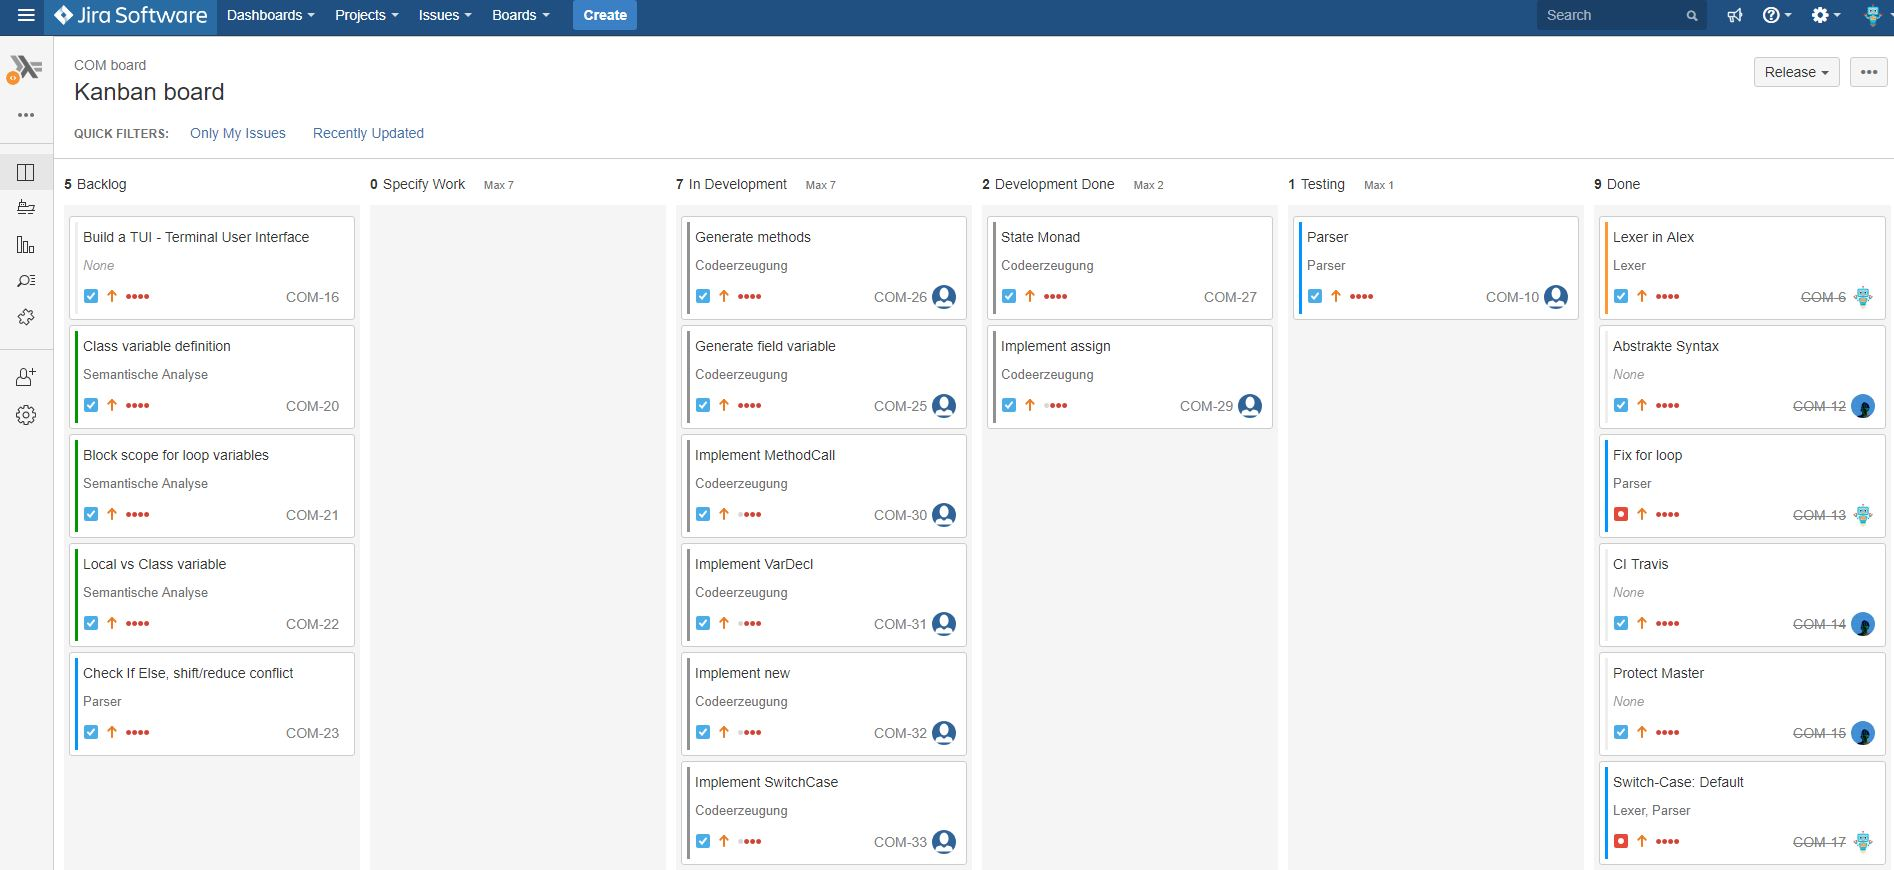
\includegraphics[scale=0.25]{images/jira.jpg}

\end{frame}

	\input{content/abstrakte-syntax.tex}
	\section{Test-Framework}

\begin{frame}{Test-Framework}
Das Test-Framework wurde selbst implementiert. Es enthält diverse Funktionen zum automatisierten überprüfen der Testfälle.

\par \medskip

Tests werden in korrekte und falsche Testfälle unterteilt.


\end{frame}

\begin{frame}[fragile]
	\frametitle{Test-Suite: Token-Coverage \& Testfälle}
	
Die Test-Suite umfasst eine Token-Coverage von 100\%. 

\par \medskip

Zusätzlich umfasst die Test-Suite insgesamt 21 gültige und 12 ungültige Testfälle.

\par \medskip

Ungültige Testfälle werden in Syntaxfehler (Parser) und Typfehler (Typchecker) unterschieden.
\end{frame}

\begin{frame}{Test-Suite: Testfälle}

Jedes Testfile liegt in einem Ordner (Correct bzw. Wrong) mit zugehöriger .java-Datei. 	

\par \medskip

Ein Testfile besteht aus: 

\begin{itemize}
	\item Erwarteten Tokens
	\item Erwarteter abstrakter Syntax
	\item Erwarteter getypter abstrakter Syntax
\end{itemize}

Zusätzlich zum eigentlichen Testfile enthält der Ordner ein ClassFile in Haskell, mit der zu erwartenden Struktur des erzeugten Classfiles.
\end{frame}

\begin{frame}[fragile]
\frametitle{Test-Suite: Beispiel Testfile}
\begin{lstlisting}[language=Haskell]
module  Correct.EmptyClass.Steps where

import           ABSTree
import           Lexer.Token

emptyTokens = [Lexer.Token.CLASS,
              Lexer.Token.IDENTIFIER "Test",
              Lexer.Token.LEFT_BRACE,
              Lexer.Token.RIGHT_BRACE
              ]

emptyABS = [Class "Test" [] []]
emptyTypedABS = [Class "Test" [] []]	
\end{lstlisting}
	
\end{frame}

\begin{frame}{Test-Suite: Beispielprogramme}
Die Testsuite enthält neben den Testfällen auch eine Reihe von (realistischeren) Anwendungsprogrammen. Diese wurden mit 'normalen' Javaprogrammen getestet.

\begin{itemize}
	\item Multiplikation
	\item Gaußsumme (kleiner Gauß)
	\item Fakultät
	\item Fibonacci
\end{itemize}	
\end{frame}



	\section{Parser}

\begin{frame}
	\frametitle{Lexer}
\end{frame}

\begin{frame}[fragile]
	\frametitle{Parser - Operatoren Priorität}
	\begin{lstlisting}
%right in
%right ASSIGN ADD ...
%right QUESTIONMARK COLON
%left OR
...
%nonassoc LESSER GREATER LESSER_EQUAL...
...
%nonassoc INCREMENT DECREMENT
	\end{lstlisting}
\end{frame}

\begin{frame}[fragile]
	\frametitle{Struktur Happy File}
	\begin{lstlisting}[basicstyle=\tiny]
		
Program
    : Class                { [$1] }
    | Program Class        { $1 ++ [$2] }
    | Program SEMICOLON    { $1 }

Statement
    : SingleStatement SEMICOLON             { $1 }
	...
    | IF LEFT_PARANTHESES Expression RIGHT_PARANTHESES
        Statement ELSE Statement
                                            { If $3 $5 (Just $7) }
    | IF LEFT_PARANTHESES Expression
        RIGHT_PARANTHESES Statement
        %prec THEN                          { If $3 $5 Nothing }
    | Switch                                { $1 }
	\end{lstlisting}
\end{frame}

\begin{frame}[fragile]
	\frametitle{Beispiel}
	\begin{lstlisting}[language=Java, basicstyle=\tiny]
class SimpleIf {
	int i;
	void doIf() {
		int a;
		a = 5;
		i = 0;
		if(a < 5) {
			i = a;
		}
		else {
			i = 2;
		}
	}
}
	\end{lstlisting}
	\begin{tikzpicture}
		\node(class){[Class \enquote{SimpleIf}]}
			child { node { FieldDecl } }
			child { node { FieldDecl } }
			;
	\end{tikzpicture}
\end{frame}

	\input{content/type-checker.tex}
	\section{Code Generator}

\begin{frame}
        \frametitle{Module}
        Die folgenden Module werden für die Erzeugung des Class files aus dem ABSTree benutzt
        \begin{itemize}
                \item genClassFile.hs
                \item genConstantPool.hs
                \item genFields.hs
                \item genMethods.hs
        \end{itemize}
\end{frame}
\begin{frame}
        \frametitle{Module}
        In den nachfolgenden Modulen sind die Datentypen enthalten die für den abstrakten Bytecode benutzt werden
        \begin{itemize}
                \item Data/Assembler.hs
                \item Data/ClassFile.hs
        \end{itemize}
        Aus dem abstrakten Bytecode wird im Module Module BinaryClass.hs der Bytecode erzeugt
\end{frame}
\begin{frame}
        \frametitle{Constanten Pool}
        Der Constantenpool ist in einer hashMap die ein Eintrag auf dessen Position abbildet.

        Im Module genConstantPool.hs sind Funktionen enthalten die ein Eintrag erzeugen und dessen Position zurückgeben bzw nur die Position zurückgeben.
\end{frame}
\begin{frame}[fragile]
        \frametitle{Beispiel genConstantPool}
        \begin{lstlisting}
genMethodRefSuper :: String
                  -> Type
                  -> State ClassFile IndexConstantPool
genMethodRefSuper name typ =
  do indexClassName <- view (super . indexSp) <$> get
     indexNameType <- genNameAndType name typ
     genInfo MethodRefInfo
               { _tagCp              = TagMethodRef
               , _indexNameCp        = indexClassName
               , _indexNameandtypeCp = indexNameType
               , _desc               = ""
               }
        \end{lstlisting}
\end{frame}
\begin{frame}[fragile]
        \frametitle{Generieren der Methoden}
        Bei der Generierung der Methoden werden auch gleichzeitig die Einträge im constanten pool erstellt.  Im State wird folgender Datentyp verwendet.
        \begin{lstlisting}
data Vars
  = Vars { _localVar :: [HM.HashMap LocVarName LocVarIndex]
         , _allLocalVar :: S.Set LocVarName
         , _classFile :: ClassFile
         , _curStack :: Int
         , _maxStack :: Int
         , _line :: LineNumber
         , _continueLine :: [LineNumber]
         }
makeLenses ''Vars
        \end{lstlisting}
\end{frame}


	% Struktur:
	% Allgemein
	% Abstrakte Syntax
	%  - Bsp. zeigen
	%  - Wie sind Typen abgebildet
	% Test framework
	%  - Aufbau des Frameworks
	%  - Bsp. ein Testfall etc.
	% Parser
	%  - Lexer aufbau
	%  - Happy File
	%  - Beispiel klasse
	% Typchecker
	%  - ...
	% Codegenerierer
	%  - ...
	% Abschließendes Beispiel

\end{document}
